\documentclass[a4paper]{article}
\usepackage[utf8]{inputenc}
\usepackage[english]{babel}
\usepackage{enumitem}	%enumerate
\usepackage{fancyhdr}	%intestazioni e piè pagina
\fancypagestyle{SE2}{% Software Engineering 2 Project Page Style
	\pagestyle{fancy}	
	%\fancyhead[LE,RO]{\slshape\rightmark}
	%\fancyhead[LO,RE]{\slshape\leftmark}
	%\fancyhead[L,R]{\slshape\rightmark}
	\cfoot{} % get rid of the page number 
	\fancyfoot[L]{\emph{PowerEnJoy}\quad \textbf{P}roject \textbf{P}lan}
	\fancyfoot[R]{\thepage}
	\renewcommand{\headrulewidth}{0.4pt}
	\renewcommand{\footrulewidth}{0.4pt}
}
\pagestyle{SE2}
%\pagestyle{fancy}
\usepackage{graphicx}	%immagini
\usepackage[colorinlistoftodos]{todonotes}	%todo
%numeri romani maiuscoli
\newcommand{\RomanNumber}[1]{\uppercase\expandafter{\romannumeral #1\relax}}
\usepackage{hyperref} %link pdf
\hypersetup{
    colorlinks,
    citecolor=black,
    filecolor=black,
    linkcolor=black,
    urlcolor=black
}
\graphicspath{{./img/}} %extra root-path for images
\usepackage[T1]{fontenc}
%\usepackage[style=alphabetic]{biblatex}
%\usepackage[babel]{csquotes}
%\usepackage[bibstyle=authortitle,citestyle=verbose-trad1]{biblatex}
%\bibliography{ITPD-main.bib}
%
\usepackage[toc,page]{appendix}
\usepackage{eurosym}%\simbolo euro
\usepackage{booktabs}%table rule
\usepackage{longtable} %multiple page tables
\usepackage{listings} 
\usepackage{multirow}

\begin{document}

\begin{titlepage}
\newcommand{\HRule}{\rule{\linewidth}{0.5mm}} % Defines a new command for the horizontal lines, change thickness here

\center % Center everything on the page
 
%----------------------------------------------------------------------------------------
%	HEADING SECTIONS
%----------------------------------------------------------------------------------------

\includegraphics[scale=0.3]{logo_poli.png}\\[0.5cm] % Include a department/university logo - this will require the graphicx package
\textsc{\LARGE Politecnico di Milano}\\[2cm] % Name of your university/college
\textsc{\Large Software Engineering \RomanNumber{2} project}\\[0.5cm] % Major heading such as course name
\textsc{\large \textbf{PowerEnJoy}}\\[1.5cm] % Minor heading such as course title

%----------------------------------------------------------------------------------------
%	TITLE SECTION
%----------------------------------------------------------------------------------------

\HRule \\[0.4cm]
{ \huge \bfseries Project Plan}\\[0.4cm] % Title of your document
\HRule \\[1.5cm]
 
%----------------------------------------------------------------------------------------
%	AUTHORS SECTION
%----------------------------------------------------------------------------------------

\begin{minipage}{0.4\textwidth}
\begin{flushleft} \large
\emph{Authors:}\\
Davide \textsc{Piantella}\\
Mario \textsc{Scrocca}\\
Moreno R. \textsc{Vendra} % Your name
\end{flushleft}
\end{minipage}
~
\begin{minipage}{0.4\textwidth}
\begin{flushright} \large
\emph{Professor:} \\
Luca \textsc{Mottola} % Supervisor's Name
\end{flushright}
\end{minipage}\\[2cm]

% If you don't want a supervisor, uncomment the two lines below and remove the section above
%\Large \emph{Author:}\\
%John \textsc{Smith}\\[3cm] % Your name

%----------------------------------------------------------------------------------------
%	DATE SECTION
%----------------------------------------------------------------------------------------

{\large January 22, 2017}\\[0.5cm] % Date, change the \today to a set date if you want to be precise
{\large version 1.0}\\[2cm]
 
%----------------------------------------------------------------------------------------

\vfill % Fill the rest of the page with whitespace
\clearpage
\end{titlepage}


%----------------------------------------------------------------------------------------
%----------------------------------------------------------------------------------------
%----------------------------------------------------------------------------------------
%----------------------------------------------------------------------------------------
%	TABLE OF CONTENTS
%----------------------------------------------------------------------------------------
\pagenumbering{Roman}
\tableofcontents
\listoffigures
\listoftables
\hypersetup{
	linkcolor=blue,
	citecolor=blue,
	urlcolor=blue
}
%----------------------------------------------------------------------------------------
%	INTRODUCTION
%----------------------------------------------------------------------------------------
\clearpage
\pagenumbering{arabic}

\section{Introduction}

\subsection{Purpose of this document}
The purpose of the \emph{Power EnJoy Project Plan} is to provide an overview of the project with respect to parameters related to the project management. This document provides an estimation of the expected size, cost and effort for the project based upon techniques that support the estimation
procedure (Function Points, COCOMO II); it also proposes a possible schedule for the project and a related allocation of resources to accomplish tasks identified and describes the possible risks related to the project presenting some possible strategies to manage them.


\subsection{Scope}
PowerEnJoy is a car-sharing service that exclusively employs electric cars; we are going to develop a web-based software system that will provide the functionalities normally provided by car-sharing services, such as allowing the user to register to the system in order to access it, showing the cars available near a given location and allowing a user to reserve a car before picking it up.
A screen located inside the car will show in real time the ride amount of money to the user. When the user reaches a predefined safe area and exits the car, the system will stop charging the user and will lock the car. The system will provide information about charging station location where the car can be plugged after the ride and incentivize virtuous behaviours of the users with discounts \cite{RASD}.

\subsection{Glossary}
The \emph{PowerEnJoy: Requirements Analysis and Specification Document} \cite{RASD}, the \emph{PowerEnJoy: Design Document} \cite{DD} and the \emph{PowerEnJoy: Integration Test Plan Document} \cite{ITPD} should be referenced for terms not defined in this section.

\subsubsection{Acronyms}
	\begin{description}
		\item [RASD:] Requirements Analysis and Specification Document
		\item [DD:] Design Document
		\item [ITPD:] Integration Test Plan Document
		\item [FP:] Function Points
		\item [ILF:] Internal logic file
		\item [EIF:] External interface file
		\item [EI:] External Input
		\item [EO:] External Output
		\item [EQ:] External Inquiries
		\item [DET:] Data Element Type
		\item [RET:] Record Element Type
		\item [FTR:] File Type Referenced
		\item [COCOMO:] COnstructive COst MOdel
		\item [SLOC:] Source Line Of Code
		\item [API:] Application Programming Interface
		\item [GPS:] Global Position System
		\item [DB:] DataBase
		\item [DBMS:] DataBase Management System
		\item [GIS:] Geographic Information System
	\end{description}
\subsubsection{Abbreviations}
	\begin{description}
		\item [w.r.t.:] with respect to
		\item [i.d.:] id est
		\item [i.f.f.:] if and only if
		\item [e.g.:] exempli gratia
		\item [etc.:] et cetera
	\end{description}

\subsection{Reference documents}
\begin{itemize}
	\item Context, domain assumptions, goals, requirements and system interfaces are all described in the \emph{PowerEnJoy: Requirements Analysis and Specification Document} \cite{RASD}
	\item Software design and architecture of the system are all described in the \emph{PowerEnJoy: Design Document} \cite{DD}
	\item System integration plan strategy is described in the \emph{PowerEnJoy: Integration Test Plan Document} \cite{ITPD}
	\item Function Point Counting Practices Manual \\ 
Release 4.3.1 International Function Point Users Group (IFPUG)
	\item Function Point Languages Table \\ 
\url{http://www.qsm.com/resources/function-point-languages-table}
	\item COCOMO II – Model Definition Manual \\
Version 2.1 Center for Software Engineering, USC

\end{itemize}


\subsection{Document overview}
This document is structured as
\begin{enumerate}
	\item \textbf{Introduction}: contains references, glossary, definitions, acronyms and abbreviations; it also explains the purpose and scope of this document
	\item \textbf{Project size, cost and effort estimation}: provides estimations of the expected size, cost and required effort of the \emph{PowerEnJoy system}
	\begin{itemize}
		\item Size estimation: \emph{Function Points} will be used to estimate the size of the \emph{PowerEnJoy system} starting from the complexity of its main functionalities
		\item Cost and effort estimation: the \emph{Constructive Cost Model (COCOMO) II} will be used to estimate the cost and effort needed to develop the \emph{PowerEnJoy system}
	\end{itemize}
	\item \textbf{Schedule}: contains a general high level schedule of the project's activities
	\item \textbf{Resource allocation}: defines how the activities in the schedule will be allocated between the members of the group
	\item \textbf{Risk management}: analyses the main risks that the project development may face and proposes the strategies to manage 
\end{enumerate}

\section{Project size, cost and effort estimation}

\subsection{Size estimation: Function Points}
\paragraph{What are FP}Given the assumption that the dimension of software can be characterized based on the functionalities that it offers, function points (FP) analysis is a process used to calculate software functional size. The most pervasive version of FP Analysis is regulated by the International Function Point User Group (IFPUG).

Functional components can be clustered as: Internal Logical Files (ILF), External Interface Files (EIF), External Inputs (EI), External Outputs (EO) and External Inquiries (EQ).

Each functional component is associated with as a \emph{complexity level} based on its associated file numbers such as: Data Element Types (DET), File Types Referenced (FTR) and Record Element Types (RET).

Each complexity level is then converted into a \emph{weight coefficient} which is used in the FP formulae to compute overall estimations.

\paragraph{Complexity levels and their weight}\autoref{tbl:complexityILF_EIF}, \autoref{tbl:complexityEI} and \autoref{tbl:complexityEO_EQ} describe how complexity level is mapped on each function component. 

In \autoref{tbl:complexityWeight} is shown how each function component is then assigned a weight
according to its complexity.


\begin{longtable}{cccc}
\toprule
\multicolumn{1}{c}{} & 
\multicolumn{3}{c}{DET}\\
\midrule
RET & 1-19 & 20-50 & 51+ \\
\midrule
1	&	Low	&	Low		&	Avg \\
2-5	&	Low	&	Avg		&	High \\
6+	&	Avg	&	High	&	High\\
\bottomrule
\caption{Complexity for ILF and EIF}
\label{tbl:complexityILF_EIF}
\end{longtable}

\begin{longtable}{cccc}
\toprule
\multicolumn{1}{c}{} & 
\multicolumn{3}{c}{DET}\\
\midrule
FTR & 1-4 & 5-15 & 16+ \\
\midrule
0-1	&	Low	&	Low		&	Avg \\
2	&	Low	&	Avg		&	High \\
3+	&	Avg	&	High	&	High\\
\bottomrule
\caption{Complexity for EI}
\label{tbl:complexityEI}
\end{longtable}

\begin{longtable}{cccc}
\toprule
\multicolumn{1}{c}{} & 
\multicolumn{3}{c}{DET}\\
\midrule
FTR & 1-5 & 6-19 & 20+ \\
\midrule
0-1	&	Low	&	Low		&	Avg \\
2-3	&	Low	&	Avg		&	High \\
4+	&	Avg	&	High	&	High\\
\bottomrule
\caption{Complexity for EO and EQ}
\label{tbl:complexityEO_EQ}
\end{longtable}


%\begin{longtable}{cccc}
%\toprule
%RET & \multicolumn{3}{c}{DET} \\
%\cmidrule(lr){2-4}
%& 1-19 & 20-50 & 51+ \\
%\midrule
%1	&	Low	&	Low		&	Avg \\
%2-5	&	Low	&	Avg		&	High \\
%6+	&	Avg	&	High	&	High\\
%\bottomrule
%\end{longtable}

\begin{longtable}{cccc}
\toprule
Component				&	Low	&	Average	&	High \\
\midrule
External Inputs			&	3	&	4		&	6 \\
External Outputs		&	4	&	5		&	7 \\
External Inquiries		&	3	&	4		&	6 \\
Internal Logic Files	&	7	&	10		&	15 \\
External Interface Files&	5	&	7		&	10 \\
\bottomrule
\caption{Function component complexity weight assignment}
\label{tbl:complexityWeight}
\end{longtable}

\paragraph{Computing FP}The Function Point (FP) is computed as
$$ FP = \sum_{i \in I} \sum_{j \in i} w_{ij}$$
where $ I = \{ILF,EIF,EI,EO,EQ\}$ and $w_{ij}$ is the weight associated with the $j$-th function component of type $i$.


\paragraph{Computing SLOC}To be able to convert FP into Source Lines Of Code (SLOC) a language-dependent factor must be taken into consideration. Since J2EE was chosen as coding language for our system, we report in \autoref{tbl:sloc_fp_j2ee} the industry gearing factor distribution of J2EE SLOC/FP factor. \cite{QSM}

\begin{longtable}{cccc}
\toprule
\textbf{Average} & \textbf{Median} & \textbf{Low} & \textbf{High}\\
\midrule
46 & 49 & 15 & 67\\
\bottomrule
\caption{J2EE SLOC/FP factor distribution}
\label{tbl:sloc_fp_j2ee}
\end{longtable}

\subsubsection{Internal Logic Files (ILFs)}

\subsubsection{External Interface Files (EIFs)}

\subsubsection{External Inputs (EIs)}

\subsubsection{External Inquiries (EQs)}
 
\subsubsection{External Outputs (EOs)} 

\subsubsection{Overall estimation}

\subsection{Cost and effort estimation: COCOMO II} 

\subsubsection{Scale Drivers}

\subsubsection{Cost Drivers}

\subsubsection{Effort equation}

\subsubsection{Schedule estimation }

\subsection{Cost and effort estimation: COCOMO II} 
COnstructive COst MOdel II (COCOMO II) is a model that allows one to estimate the cost, effort, and schedule when planning a new software development activity. COCOMO II.2000 is the latest major extension to the original \mbox{COCOMO 81} model published in 1981.

It consists of three submodels, each one offering increased fidelity the further along one is in the project planning and design process \cite{COCOMO}.

Since the system we are to develop is brand new and there is no previous system we have to adopt the \emph{early design} submodel.

\paragraph{Important note}All parameters and coefficients used in this section are formally defined in the \emph{COCOMO II.2000 Model Definition Manual} \cite{COCOMOManual}. Each cost driver and scale factor value is determined w.r.t. definition tables in the same manual that are not reported here.

\paragraph{COCOMO effort equation}\label{par:cocomoEquation}This formula estimates the project effort in Person-Months (PM)
$$PM = A \cdot Size^{E} \cdot \prod_{i \in CostDrivers}C_{i}$$
where 
\begin{itemize}
	\item $A=2.94$ approximates a productivity constant in $\frac{PM}{KiloSLOC}$
	\item $Size$ is the estimated size of the project in KiloSLOC, it can be deducted from \hyperref[sec:FPResult]{Function Points analysis}
	\item $E$ is an aggregation of five Scale Factors which is computed as $$E = 0.91 + 0.01 \cdot \sum_{j=1}^{5}{SF_j}$$
	\item $C$ is the effort multiplier derived from each Cost Driver
\end{itemize}

\clearpage

\subsubsection{Scale Factors}
Here are described the five Scale Factors of the COCOMO II model, in \autoref{tbl:cocomoSF} are specified their numerical value according to the model definition.
 
{\scriptsize
\begin{longtable}{c|cccccc}
\toprule
\specialcell{Scale\\Factors}&\specialcell{Very\\Low}&Low&Nominal&High&\specialcell{Very\\High}&\specialcell{Extra\\High}\\
\midrule
PREC	&
\specialcell{thoroughly\\unprecedented\\\textbf{6.20}} & 
\specialcell{largely\\unprecedented\\\textbf{4.96}} & 
\specialcell{somewhat\\unprecedented\\\textbf{3.72}} & 
\specialcell{generally\\familiar\\\textbf{2.48}} & 
\specialcell{largely\\familiar\\\textbf{1.24}} & 
\specialcell{thoroughly\\familiar\\\textbf{0.00}} \\
\midrule
FLEX &
\specialcell{rigorous\\\textbf{5.07}} & 
\specialcell{occasional\\relaxation\\\textbf{4.05}} & 
\specialcell{some\\relaxation\\\textbf{3.04}} & 
\specialcell{general\\conformity\\\textbf{2.03}} & 
\specialcell{some\\conformity\\\textbf{1.01}} & 
\specialcell{general\\goals\\\textbf{0.00}} \\
\midrule
RESL &
\specialcell{little\\(20\%)\\\textbf{7.07}} & 
\specialcell{some\\(40\%)\\\textbf{5.65}} & 
\specialcell{often\\(60\%)\\\textbf{4.24}} & 
\specialcell{generally\\(75\%)\\\textbf{2.83}} & 
\specialcell{mostly\\(90\%)\\\textbf{1.14}} & 
\specialcell{full\\(100\%)\\\textbf{0.00}} \\
\midrule
TEAM &
\specialcell{very\\difficult\\interactions\\\textbf{5.48}} & 
\specialcell{some\\difficult\\interactions\\\textbf{4.38}} & 
\specialcell{basically\\cooperative\\interactions\\\textbf{3.29}} & 
\specialcell{largely\\cooperative\\\textbf{2.19}} & 
\specialcell{highly\\cooperative\\\textbf{1.10}} & 
\specialcell{seamless\\interactions\\\textbf{0.00}} \\
\midrule
PMAT &
\specialcell{SW-CMM\\Level 1\\Lower\\\textbf{7.80}} & 
\specialcell{SW-CMM\\Level 1\\Upper\\\textbf{6.24}} & 
\specialcell{SW-CMM\\Level 2\\\textbf{4.68}} & 
\specialcell{SW-CMM\\Level 3\\\textbf{3.12}} & 
\specialcell{SW-CMM\\Level 4\\\textbf{1.56}} & 
\specialcell{SW-CMM\\Level 5\\\textbf{0.00}} \\
\bottomrule
\caption{\label{tbl:cocomoSF}COCOMO II scale factors values}
\end{longtable}
}

\paragraph{Precedentedness - PREC} It is high if a product is similar to several projects previously developed by the team. Since we do not have ever develop such a big project, although we have largely understood the product objectives and there is a minimal need of innovative algorithms or innovative data processing architectures, we decide that
\DadoCenter{PREC is \textbf{LOW}}

\paragraph{Development Flexibility - FLEX} It is high if there are no specific constraints to conform to pre-established requirements and external interface specifications. The italian law establishes specific constraints regarding the characteristics and usage of car sharing systems, driving licenses and privacy policy. Requirements specified by the client do not excessively restrict the development process, some external APIs should used in order to fulfill the requirements.\\We decide that
\DadoCenter{FLEX is \textbf{NOMINAL}}

\paragraph{Risk Resolution - RESL} It is high if the project has a good risk management plan, clear definition of budget and schedule, focus on architectural definition. The \hyperref[sec:riskManagement]{Risk Management Plan} identifies generally all critical risk items and determines actions in order to resolve them. As specified in the \hyperref[sec:schedule]{Schedule section} a relevant portion of development process is devoted to establishing architecture, given general product objectives.\\Therefore we decide that
\DadoCenter{RESL is \textbf{HIGH}}

\paragraph{Team Cohesion - TEAM} It is high if all project development team members are able to work in a team and share the same vision and commitment. As objectives, cultures, ages and backgrounds are the same for all team members we decide that
\DadoCenter{TEAM is \textbf{VERY HIGH}}

\paragraph{Project Maturity - PMAT} It reflects the CMMI index of the project. Since this project can be considered a managed process, planned and executed according to policies with the usage of adequate and planned resources, stakeholders constantly involved in incremental product reviews, we decide that the CMMI index is Level 2: Managed at the Project Level, therefore
\DadoCenter{PMAT is \textbf{NOMINAL}}

\paragraph{E parameter}In the \autoref{tbl:SFChosenValues} are reported the values chosen for the five Scale Factors
\begin{longtable}{ccc}
\toprule
Scale Factor&Value&Numerical Value\\
\midrule
PREC&Low&4.96\\
FLEX&Nominal&3.04\\
RESL&High&2.83\\
TEAM&Very High&1.10\\
PMAT&Nominal&4.68\\
\midrule
\multicolumn{2}{c}{\textbf{Total}}&\textbf{16.61}\\
\bottomrule\\
\caption{\label{tbl:SFChosenValues}Scale factors chosen values}
\end{longtable}
The $E$ parameter of \hyperref[par:cocomoEquation]{COCOMO effort equation} is computed as
$$E = 0.91 + 0.01 \cdot \sum_{j=1}^{5}{SF_j} = 0.91+0.01\cdot 16.61 = 1.0761$$


\subsubsection{Cost Drivers}
Since we refer to the \emph{Early Design} model of COCOMO II, the cost drivers are obtained averaging their \emph{Post-Architecture} counterparts as shown in \autoref{tbl:costDriverConversion}.
\begin{longtable}{ll}
\toprule
\specialcell{Early Design\\Cost Drivers} & \specialcell{Combined Post-Architecture\\Cost Drivers}\\
\midrule
PERS&ACAP, PCAP, PCON\\
RCPX&RELY, DATA, CPLX, DOCU\\
RUSE&RUSE\\
PDIF&TIME ,STOR, PVOL\\
PREX&APEX, PLEX, LTEX\\
FCIL&TOOL, SITE\\
SCED&SCED\\
\bottomrule\\
\caption{\label{tbl:costDriverConversion}Cost drivers conversion}
\end{longtable}

\begin{longtable}{l|ccccccc}
\toprule
\specialcell{Cost\\Driver}&\specialcell{Extra\\Low}&\specialcell{Very\\Low}&Low&Nominal&High&\specialcell{Very\\High}&\specialcell{Extra\\High}\\
\midrule
PERS &2.12 &1.62 &1.26 &1.00 &0.83 &0.63 &0.50\\
RCPX &0.49 &0.60 &0.83 &1.00 &1.33 &1.91 &2.72\\
RUSE &-	   &-	 &0.95 &1.00 &1.07 &1.15 &1.24\\
PDIF &-	   &-    &0.87 &1.00 &1.29 &1.81 &2.61\\
PREX &1.59 &1.33 &1.22 &1.00 &0.87 &0.74 &0.62\\
FCIL &1.43 &1.30 &1.10 &1.00 &0.87 &0.73 &0.62\\
SCED &-	   &1.43 &1.14 &1.00 &1.00 &1.00 &-\\
\bottomrule
\caption{\label{tbl:costDriverConversionValue}COCOMO II early design cost driver values}
\end{longtable}

\paragraph{Personnel Capability - PERS}
\begin{itemize}
	\item \textbf{Analyst Capability - ACAP}: Analysts are personnel who work on requirements, high-level design and detailed design. Since we consider ourselves as good analysts, with the ability to communicate and cooperate, we consider this parameter as \textbf{HIGH}.
	\item \textbf{Programmer Capability - PCAP}: This parameter reflect the capability of the programmers as a team rather than as individuals. Since all team members have already done with profit several team projects before, we consider this parameter as \textbf{HIGH}.
	\item \textbf{Personnel Continuity - PCON}: The rating scale is in terms of the project’s annual personnel turnover. Since the team is composed of 3 members and the average turnover is 2 years, this parameter is \textbf{VERY LOW}.
\end{itemize}

\begin{longtable}{ccc}
\multicolumn{3}{c}{\textbf{PERS}}\\
\toprule
Cost Driver&Value&Numerical Value\\
\midrule
ACAP&High&4\\
PCAP&High&4\\
PCON&Very Low&1\\
\midrule
\multicolumn{2}{c}{\textbf{Total}}&\textbf{9}\\
\bottomrule
\end{longtable}

Therefore PERS is \textbf{NOMINAL}.

\paragraph{Product Reliability and Complexity - RCPX}
\begin{itemize}
	\item \textbf{Required Software Reliability - RELY} This is the measure of the extent to which the software must perform its intended function over a period of time. If the effect of a software failure is only slight inconvenience then RELY is very low. Since a product failure will cause high financial loss to our client's core business, this parameter is \textbf{HIGH}.
	\item \textbf{Data Base Size - DATA} This cost driver attempts to capture the effect large test data requirements have on product development. The rating is determined by calculating D/P, the ratio of bytes in the testing database to SLOC in the program. Given the project specifications we estimate a testing database size of 10Mb and the \hyperref[sec:FPResult]{FP analysis} estimates SLOC between 7728 and 11256, the D/P ratio is between 932 and 1357. Therefore this parameter is \textbf{HIGH}.
	\item \textbf{Product Complexity - CPLX} Complexity is divided into five areas: control operations, computational operations, device-dependent operations, data management operations, and user interface management operations.
	\begin{itemize}
		\item User interface management: simple use of widget set. It is NOMINAL.
		\item Data management operations: large operational database with many updates, possibly with triggers, multi-file structured inputs, data restructuring. It is HIGH.
		\item Device dependent Operations: I/O processing includes device selection, status checking and error processing. It is NOMINAL.
		\item Computational operations: Use of standard math, basic matrix and vector operations. It is NOMINAL.
		\item Control operations: Reentrant and recursive coding. Task synchronization, complex callbacks. It is VERY HIGH.
	\end{itemize}
	Due to this analysis, the CPLX parameter is \textbf{NOMINAL}.
	\item \textbf{Documentation Match to Life Cycle Needs - DOCU} This cost driver is evaluated in terms of the suitability
of the project's documentation. Since the documentation of the project is supposed to be right-sized to life cycle needs, this parameter is \textbf{NOMINAL}
\end{itemize}

\begin{longtable}{ccc}
\multicolumn{3}{c}{\textbf{RCPX}}\\
\toprule
Cost Driver&Value&Numerical Value\\
\midrule
RELY&High&4\\
DATA&High&4\\
CPLX&Nominal&3\\
DOCU&Nominal&3\\
\midrule
\multicolumn{2}{c}{\textbf{Total}}&\textbf{14}\\
\bottomrule
\end{longtable}

Therefore RCPX is \textbf{HIGH}.

\paragraph{Developed for Reusability - RUSE} This cost driver accounts for the additional effort needed to construct components intended for reuse on current or future projects. This effort is consumed with creating more generic design of software, more elaborate documentation, and more extensive testing to ensure components are ready for use in other applications.

Since some project components must cover general aspects of different possible software projects, this parameter is \textbf{NOMINAL}.

\paragraph{Platform Difficulty - PDIF}
\begin{itemize}
	\item \textbf{Execution Time Constraint - TIME} This is a measure of the execution time constraint imposed upon a software system. The rating is expressed in terms of the percentage of available execution time expected to be used by the system or subsystem consuming the execution time resource. Since the system may have exceptional spikes of usage, the idle resource allocation should not exceed 70\% of available execution time. Therefore this parameter is \textbf{HIGH}.
	\item \textbf{Main Storage Constraint - STOR} This rating represents the degree of main storage constraint imposed on a software system or subsystem. Since the system will not require an incremental disk space except for the database whose size is trivial w.r.t modern disk capacity, this parameter is \textbf{NOMINAL}.
	\item \textbf{Platform Volatility - PVOL} \emph{Platform} is used here to mean the complex of hardware and software the product calls on to perform its tasks. Our system may use a web server, a DBMS and some external APIs, we expect major releases of them every 6 months and minor releases every 2 weeks, therefore this parameter is \textbf{NOMINAL}.
\end{itemize}

\begin{longtable}{ccc}
\multicolumn{3}{c}{\textbf{PDIF}}\\
\toprule
Cost Driver&Value&Numerical Value\\
\midrule
TIME&High&4\\
STOR&Nominal&3\\
PVOL&Nominal&3\\
\midrule
\multicolumn{2}{c}{\textbf{Total}}&\textbf{10}\\
\bottomrule
\end{longtable}

Therefore PDIF is \textbf{NOMINAL}.

\paragraph{Personnel Experience - PREX}
\begin{itemize}
	\item \textbf{Applications Experience - APEX} The rating for this cost driver is dependent on the level of applications experience of the project team developing the software system. Since all members of the team have an equivalent level of experience with this type of application which is approximately 4 months, this parameter is \textbf{VERY LOW}.
	
	\item \textbf{Platform Experience - PLEX} This parameter reflect the ability to understand and use powerful platforms, including more graphic user interface, database, networking and so on. Since all members of the team have already deal (in different teams) with projects that relied on platforms similar to the ones that will be used for the PowerEnJoy project for an average period of 2 years, this parameter is set to \textbf{NOMINAL}.
	
	\item \textbf{Language and Tool Experience - LTEX} This is a measure of the level of programming language and software tool experience of the project team developing the software system or subsystem. All team members have quite good knowledge of many development best practices and software tools that will be used such as version control systems, integrated development environments, testing frameworks, development quality control software, etc. None of team members have any experience regarding J2EE. All these things considered, this parameter is \textbf{NOMINAL}.
	
\end{itemize}

\begin{longtable}{ccc}
\multicolumn{3}{c}{\textbf{PREX}}\\
\toprule
Cost Driver&Value&Numerical Value\\
\midrule
APEX&Very Low&1\\
PLEX&Nominal&3\\
LTEX&Nominal&3\\
\midrule
\multicolumn{2}{c}{\textbf{Total}}&\textbf{7}\\
\bottomrule
\end{longtable}

Therefore PREX is \textbf{LOW}.

\paragraph{Facilities - FCIL}
\begin{itemize}
	\item \textbf{Use of Software Tool - TOOL} Software development tools will be used during the whole development cycle (version control systems, integrated development environments, testing frameworks, development quality control software, bug report systems, virtual team desks, etc.), therefore this parameter is \textbf{NOMINAL}.
	\item \textbf{Multisite Development - SITE} Since all team members and stakeholders live in the same metropolitan area, this parameter is \textbf{HIGH}.
\end{itemize}

\begin{longtable}{ccc}
\multicolumn{3}{c}{\textbf{FCIL}}\\
\toprule
Cost Driver&Value&Numerical Value\\
\midrule
TOOL&Nominal&3\\
SITE&High&4\\
\midrule
\multicolumn{2}{c}{\textbf{Total}}&\textbf{7}\\
\bottomrule
\end{longtable}

Therefore FCIL is \textbf{High}.

\paragraph{Required Development Schedule - SCED}\label{par:sced}
This rating measures the schedule constraint imposed on the project team developing the software. Since the schedule considers mandatory deadlines, there should not be any compression or expansion for the whole project (\emph{i.d. 100\% of nominal schedule)}, therefore this parameter is set to \textbf{NOMINAL}.

\clearpage
\paragraph{Cost Drivers summary}
In \autoref{tbl:CDChosenValues} is reported the value of each cost driver as determined in this section and the corresponding effort multiplier as specified in \autoref{tbl:costDriverConversionValue}.

\begin{longtable}{lcc}
\specialcell{Cost\\Driver} & Value & \specialcell{Numerical Value\\\emph{(Effort Multiplier)}}\\
\midrule
PERS&Nominal&1.00\\
RCPX&High&1.33\\
RUSE&Nominal&1.00\\
PDIF&Nominal&1.00\\
PREX&Low&1.22\\
FCIL&High&0.87\\
SCED&Nominal&1.00\\
\bottomrule
\caption{\label{tbl:CDChosenValues}Cost drivers effort multipliers}
\end{longtable}


\subsubsection{Effort equation}
The COCOMO II \hyperref[par:cocomoEquation]{effort equation} can now be computed as
\begin{align*}
PM &= A \cdot Size^{E} \cdot \prod_{i \in CostDrivers}C_{i} \\
&= 2.94 \cdot Size^{1.0761} \cdot (1 \cdot 1.33 \cdot 1 \cdot 1 \cdot 1.22 \cdot 0.87 \cdot 1)\\
&= 2.94 \cdot Size^{1.0761} \cdot 1.4112\\
\end{align*}

Therefore
$$PM_{avg} = 2.94 \cdot 7.728^{1.0761} \cdot 1.4112 = 37$$

$$PM_{max} = 2.94 \cdot 11.256^{1.0761} \cdot 1.4112 = 56$$
\subsubsection{Schedule estimation} 
According to the model definition, the duration D (in months) of the project can be estimated as
$$D = 3.67 \cdot (PM_{NS})^F \cdot \frac{SCED\%}{100}$$
where
\begin{itemize}
	\item $PM_{NS}$ is the Person-Months estimation without considering the SCED cost driver
	\item $F = 0.28 + 0.2 \cdot (E-0.91)$
	\item $E$ is the aggregation of scale factors previously determined
	\item $SCED\%$ is the SCED nominal value percentage, in our case is set to $100\%$ (see \hyperref[par:sced]{SCED paragraph})
\end{itemize}

Since the effort multiplier of SCED cost driver is $1$, in our case $$PM_{NS} = PM$$
Since as previously specified $E = 1.0761$ we can compute $$F = 0.28+0.2 \cdot (1.0761-0.91) = 0.31322$$
Therefore
\begin{align*}
D_{avg} &= 3.67 \cdot 37^{0.31322} \cdot 1 = 11.373 \text{ months}\\
D_{max} &= 3.67 \cdot 56^{0.31322} \cdot 1 = 12.949 \text{ months}
\end{align*}


\section{Schedule}\label{sec:schedule}
In this section the schedule for the \emph{PowerEnJoy} project will be presented; it is a high-level general schedule that allows the reader to understand the main phases of the project specification and development.

\subsection{Notes for the charts}
\subsubsection{\hyperref[fig:rasdGantt]{RASD Gantt chart (\autoref{fig:rasdGantt})}}
\begin{itemize}
	\item \textbf{Meetings with client}: all the resources will be present at the meeting
	\item \textbf{Modelization of the World and the Machine}: this part requires discussion and cooperation, hence it will be assigned to all the resources
	\item \textbf{Identification of use cases}: Davide will start working on this activity in date 28/10/2016
	\item \textbf{In progress meeting with client}: all the resources will be present at the meeting
	\item \textbf{Requirements refinement}: the requirements will be updated based on updates made in other parts of the document, during its development
	\item \textbf{Alloy modelization}: Davide will start working on this activity in date 05/11/2016
	\item \textbf{Document revision}: these days are left for the revision of the document and to complete tasks that eventually need more time
\end{itemize}

\subsubsection{\hyperref[fig:ddGantt]{DD Gantt chart (\autoref{fig:ddGantt})}}
\begin{itemize}
	\item \textbf{Architecture draft}: this part requires discussion and cooperation, hence it will be assigned to all the resources
	\item \textbf{Meeting with clients}: all the resources will be present at the meeting
	\item \textbf{Sequence diagrams}: Moreno will start working on this activity in date 29/11/2016
\end{itemize}

\subsubsection{\hyperref[fig:itpdGantt]{ITPD Gantt chart (\autoref{fig:itpdGantt})}}
\begin{itemize}
	\item \textbf{Integration test strategy and Definition of precedences}: these initial tasks will be accomplished at the same time and since they require discussion and cooperation, they will be assigned to all the resources
	\item \textbf{Document revision}: Davide will start working on this activity in date 19/12/2016
\end{itemize}

\subsubsection{\hyperref[fig:devGantt]{Development Gantt chart (\autoref{fig:devGantt})}}
All of the tasks in this chart refers to high level activities; more specific charts will be produces during the development phase.

\begin{figure}[h]
	\centering
	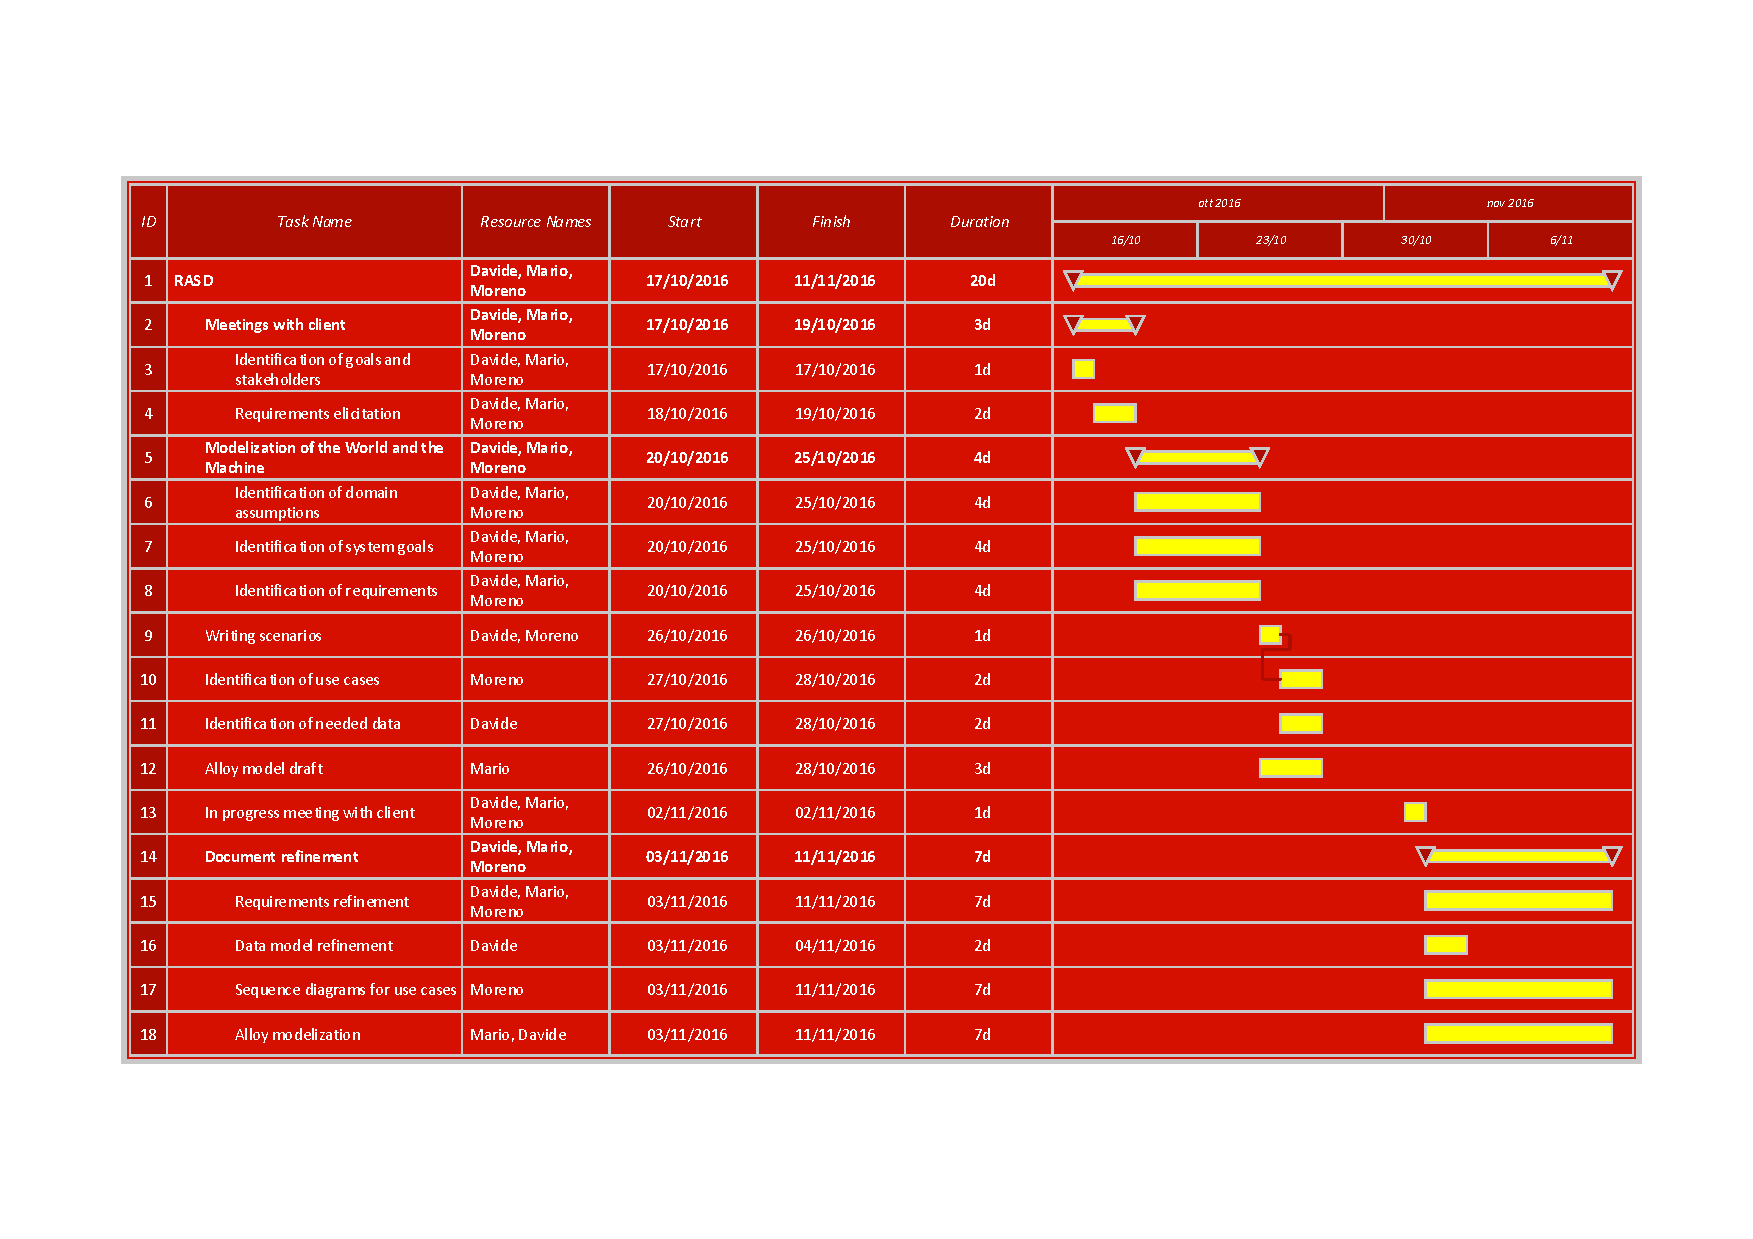
\includegraphics[angle=90, width=\linewidth]{RASDGantt}	\caption{
		\label{fig:rasdGantt} 
		RASD Gantt chart
	}
\end{figure}

\begin{figure}[h]
	\centering
	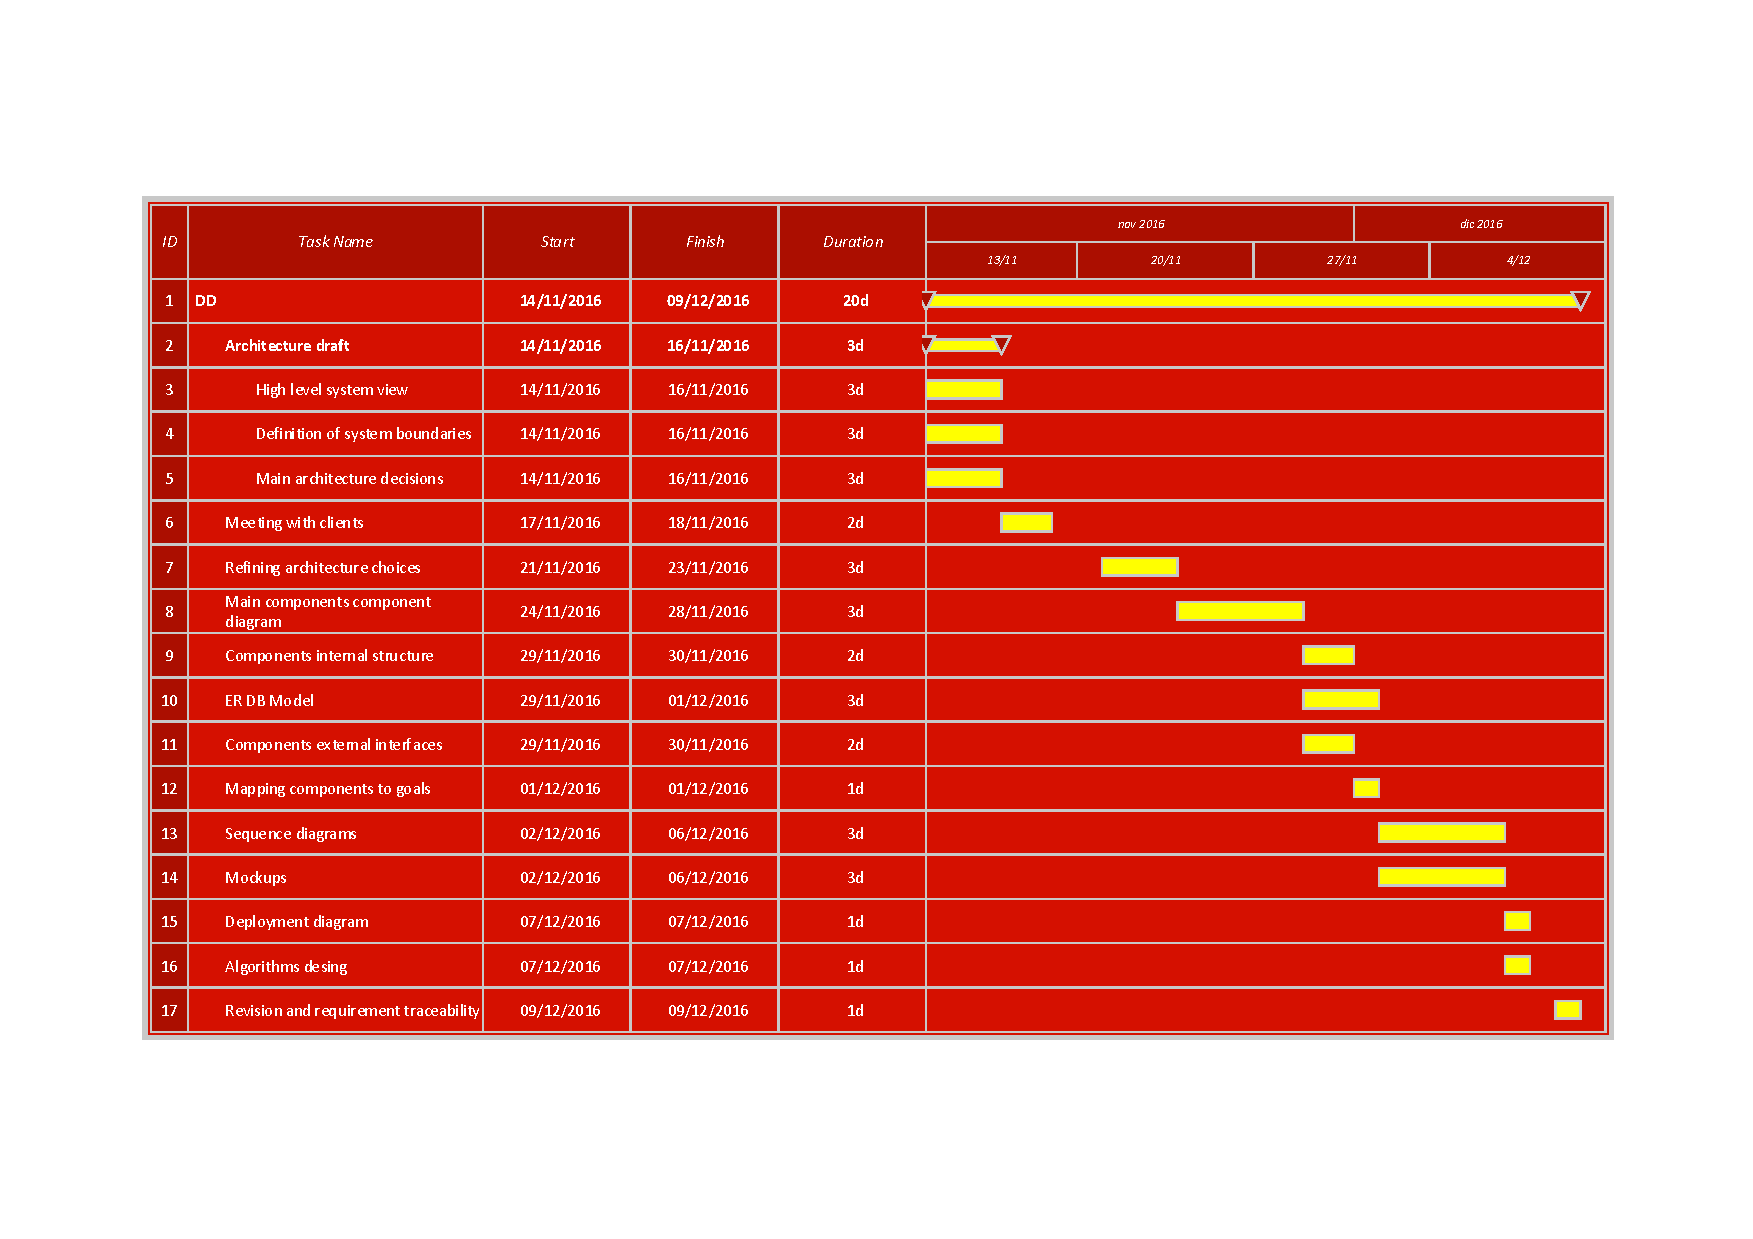
\includegraphics[angle=90, width=\linewidth]{DDGantt}	\caption{
		\label{fig:ddGantt} 
		DD Gantt chart
	}
\end{figure}

\begin{figure}[h]
	\centering
	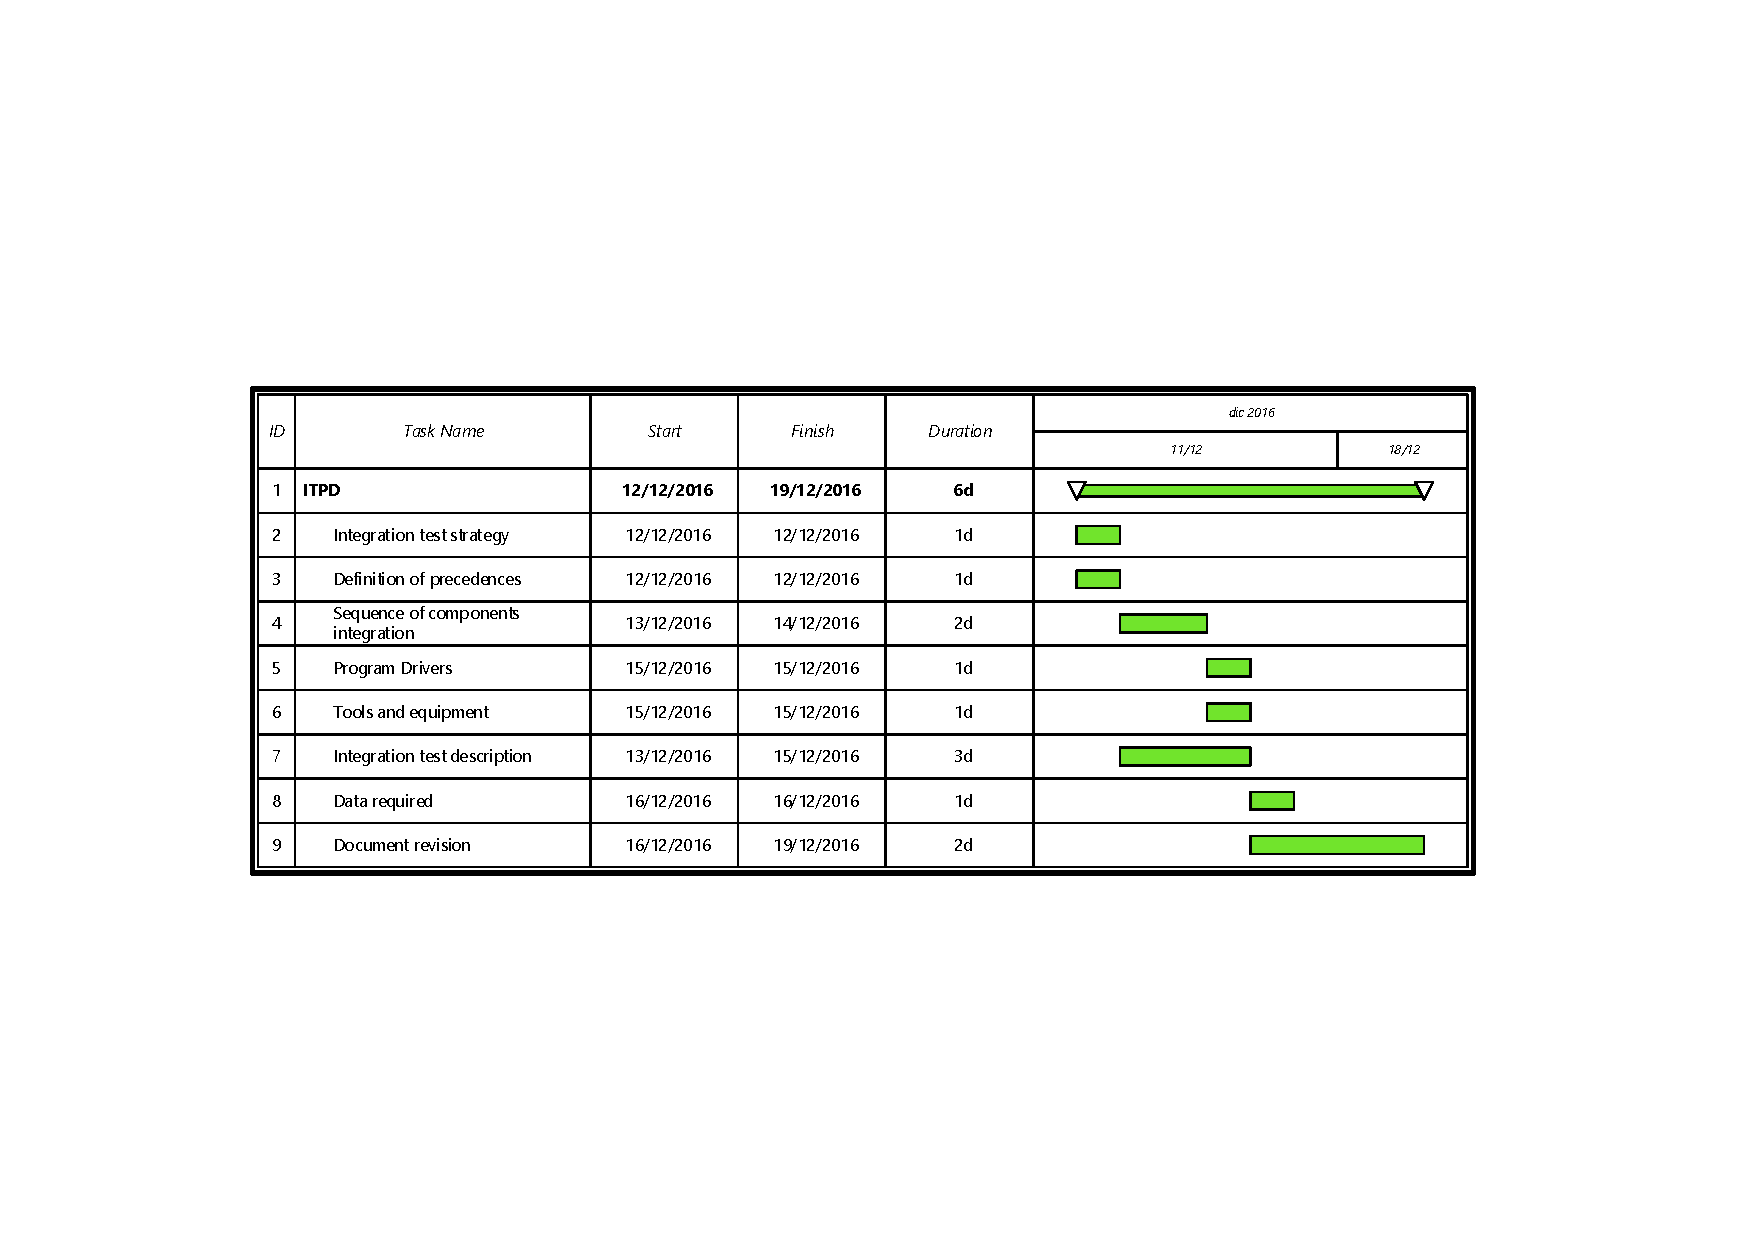
\includegraphics[angle=90, width=\linewidth]{ITPDGantt}	\caption{
		\label{fig:itpdGantt} 
		ITPD Gantt chart
	}
\end{figure}

\begin{figure}[h]
	\centering
	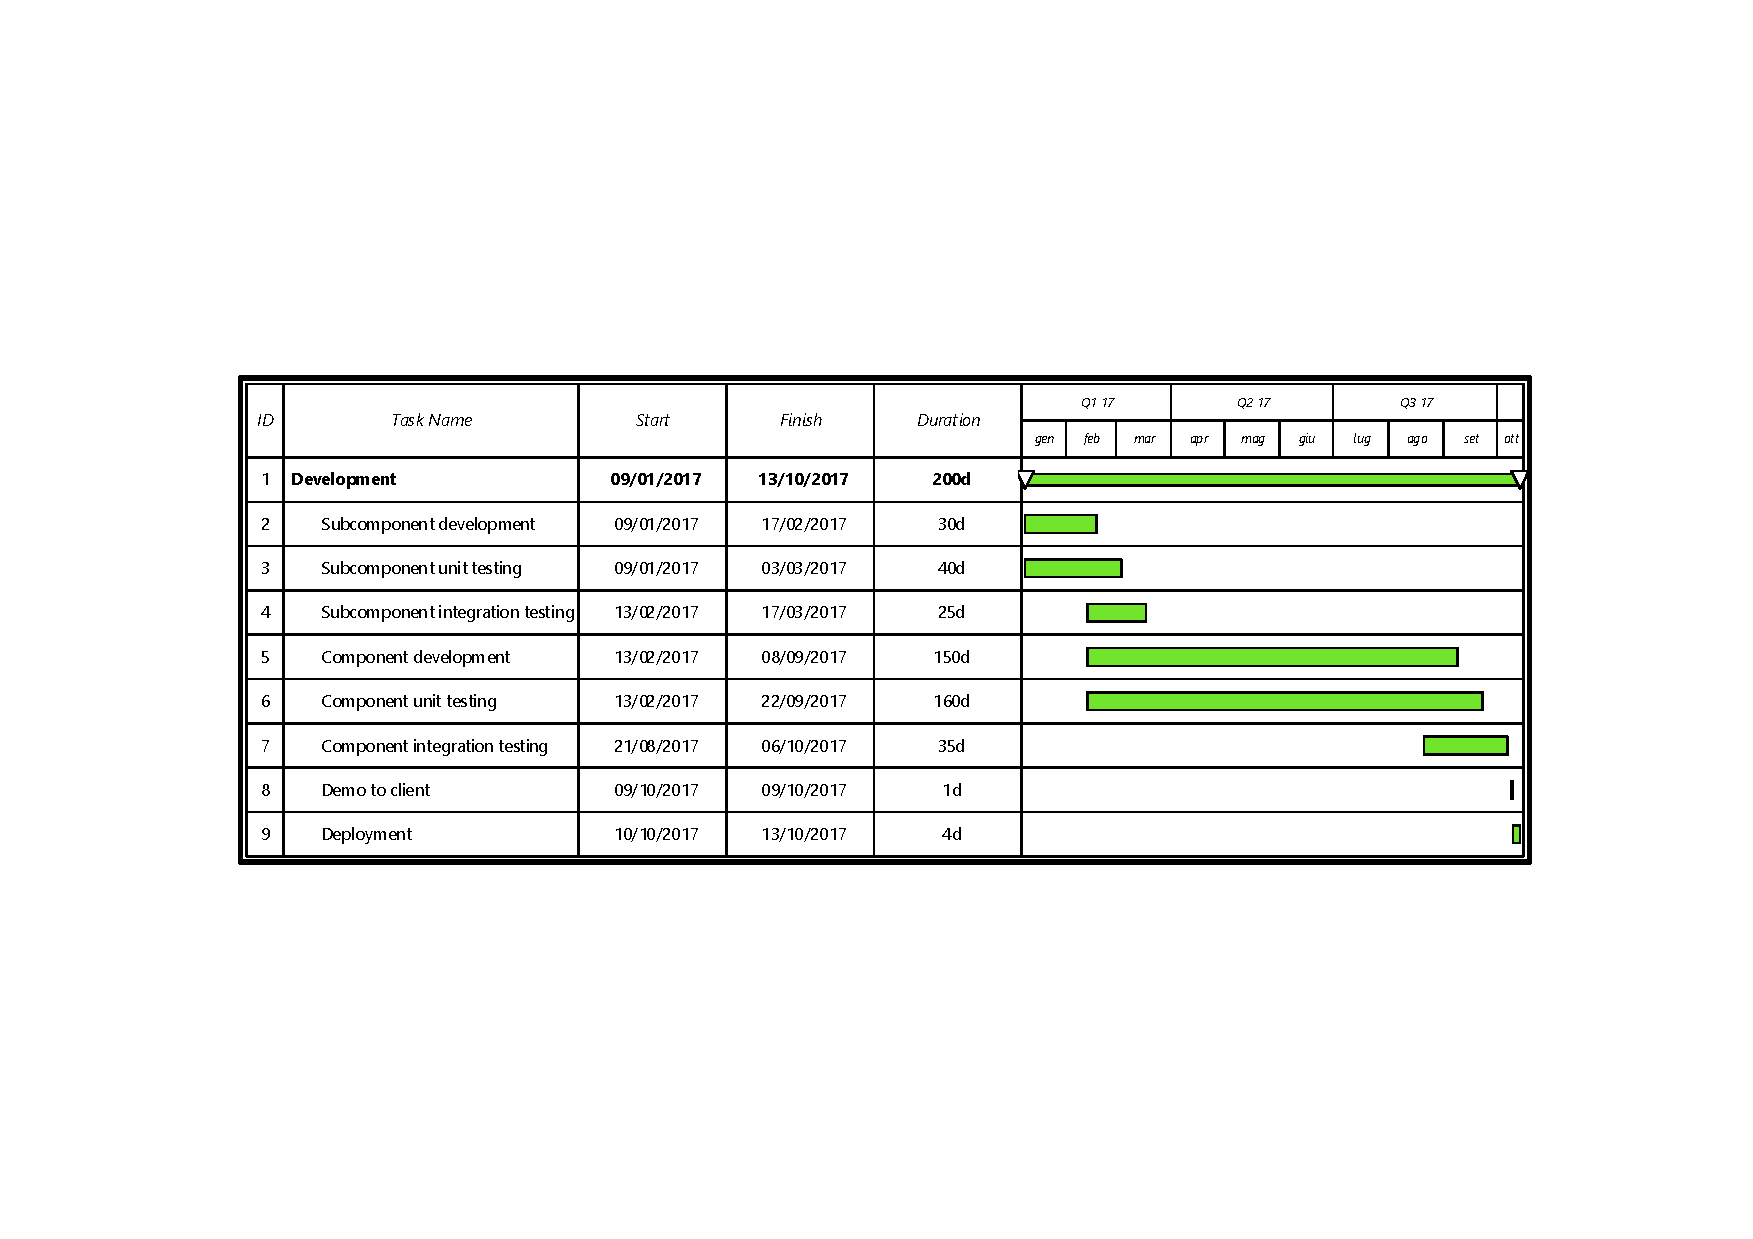
\includegraphics[angle=90, width=\linewidth]{DevGantt}	\caption{
		\label{fig:devGantt} 
		Development Gantt chart
	}
\end{figure}

\clearpage


\section{Resources Allocation}\label{sec:resAlloc}
In this section the resource allocation for the tasks related to \emph{PowerEnJoy project} will be presented; it uses the high level tasks shown in section \ref{sec:schedule} to show which tasks will be assign to each of the team members.

\begin{figure}[h]
	\centering
	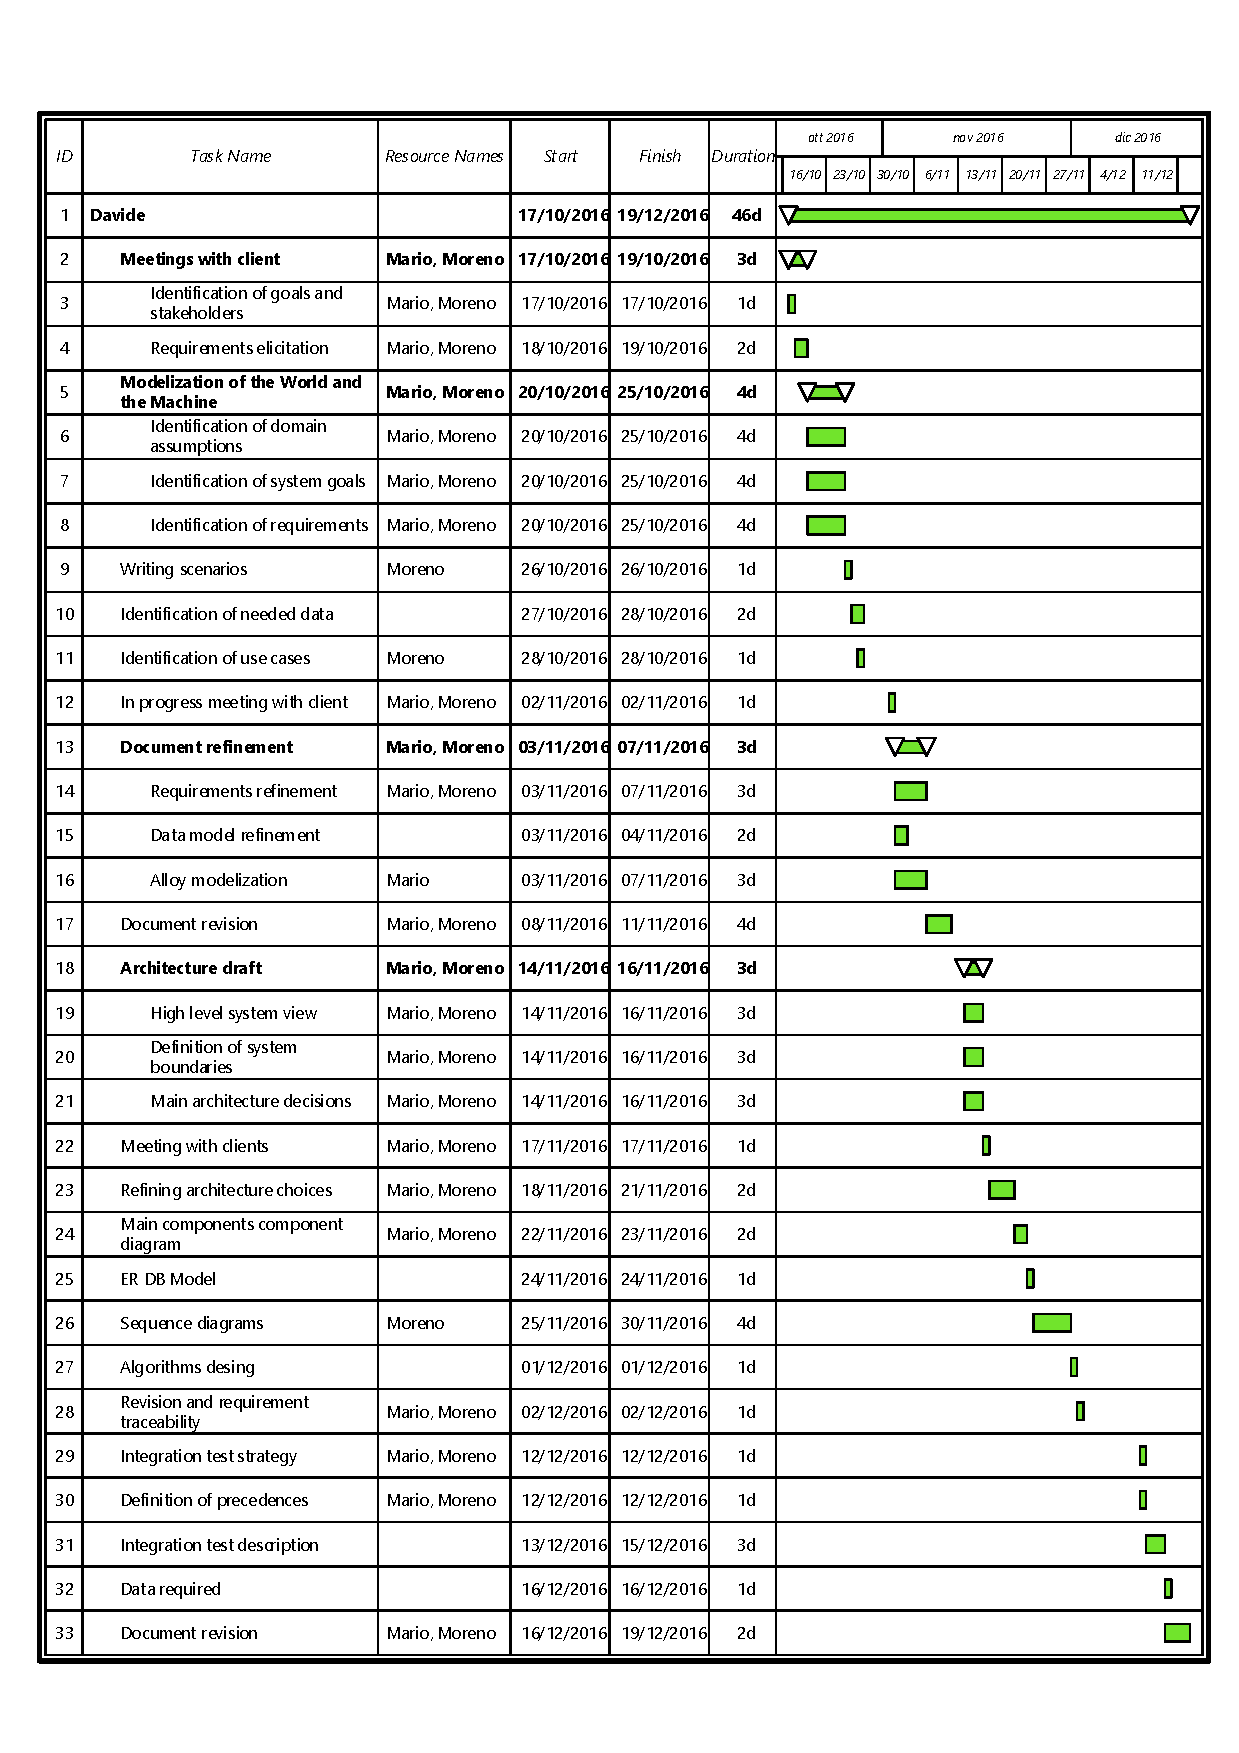
\includegraphics[width=\linewidth]{DavideGantt}	\caption{
		\label{fig:davideGantt} 
		Davide Piantella tasks Gantt chart
	}
	
\end{figure}\begin{figure}[h]
	\centering
	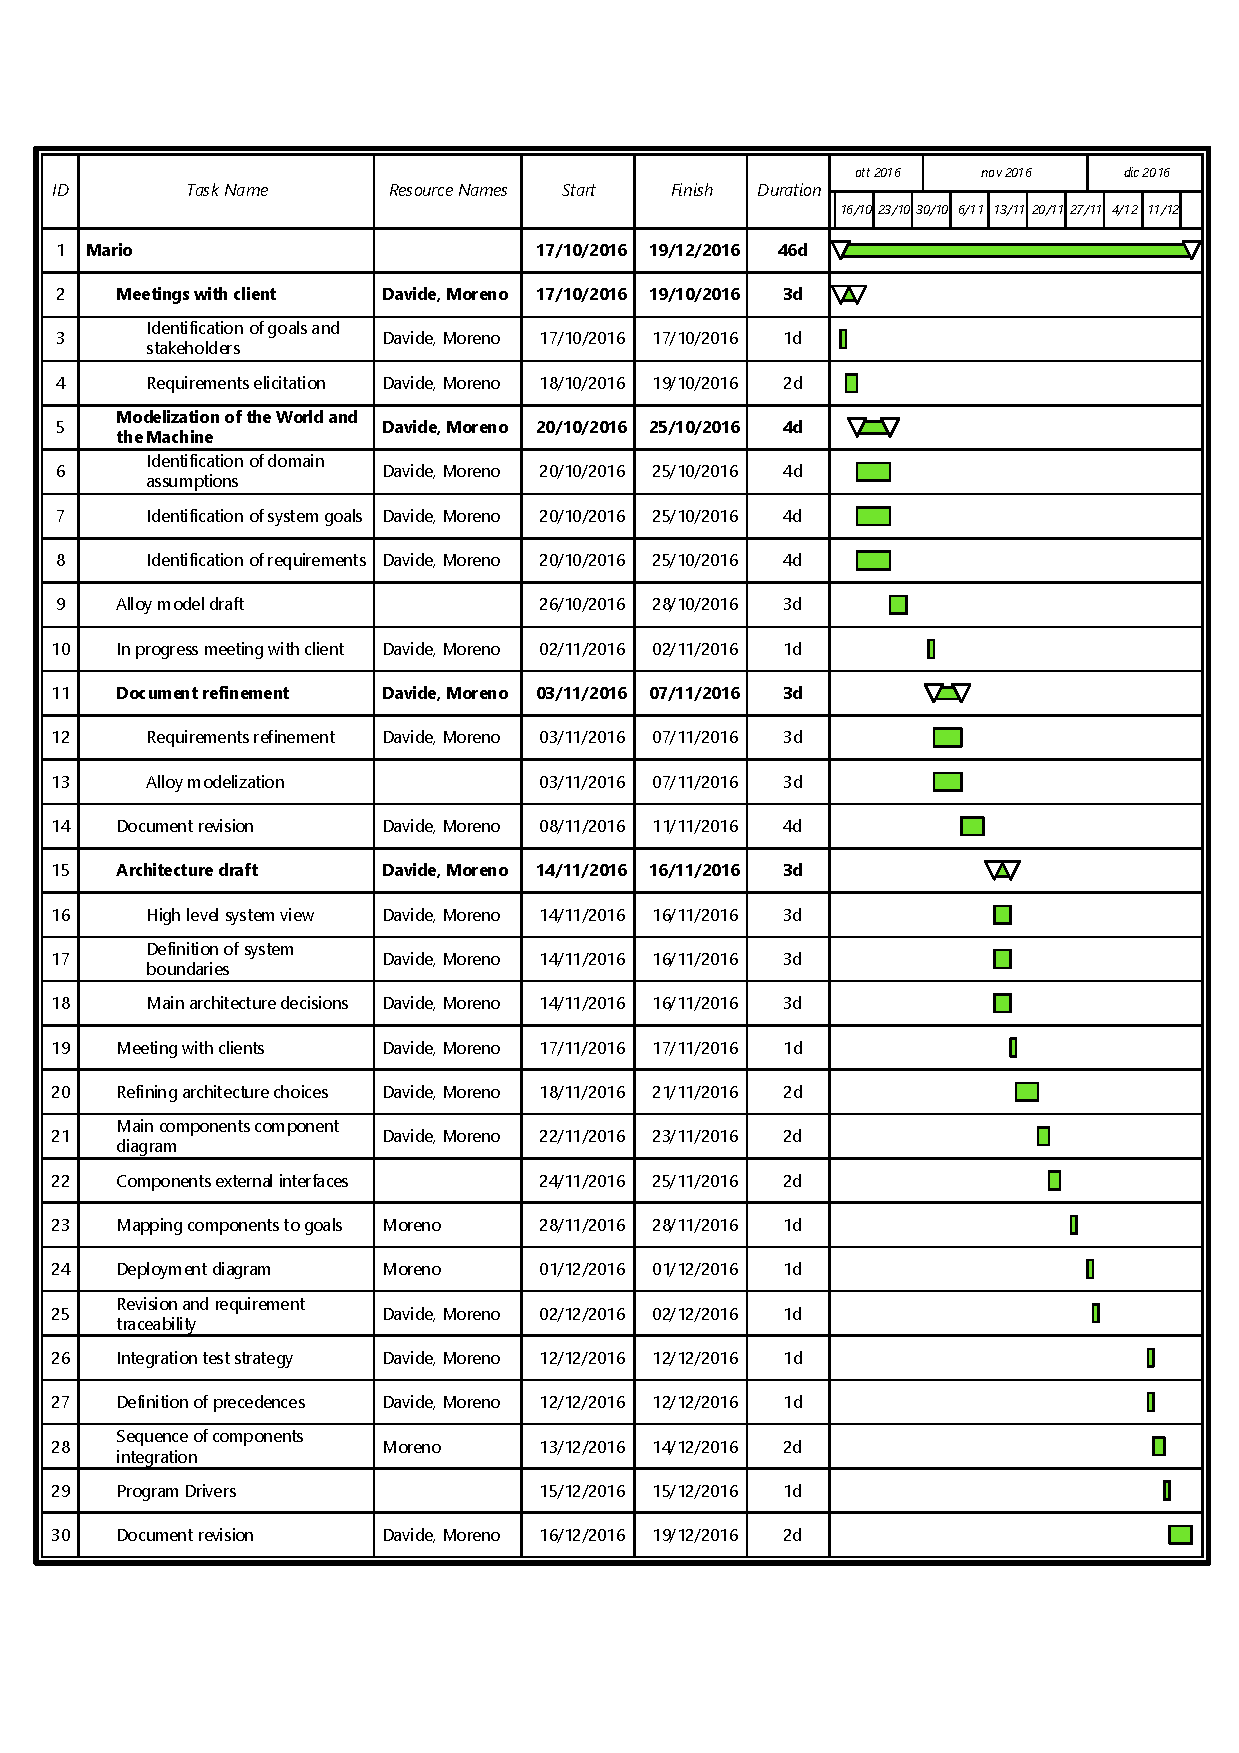
\includegraphics[width=\linewidth]{MarioGantt}	\caption{
		\label{fig:marioGantt} 
		Mario Scrocca tasks Gantt chart
	}
	
\end{figure}\begin{figure}[h]
	\centering
	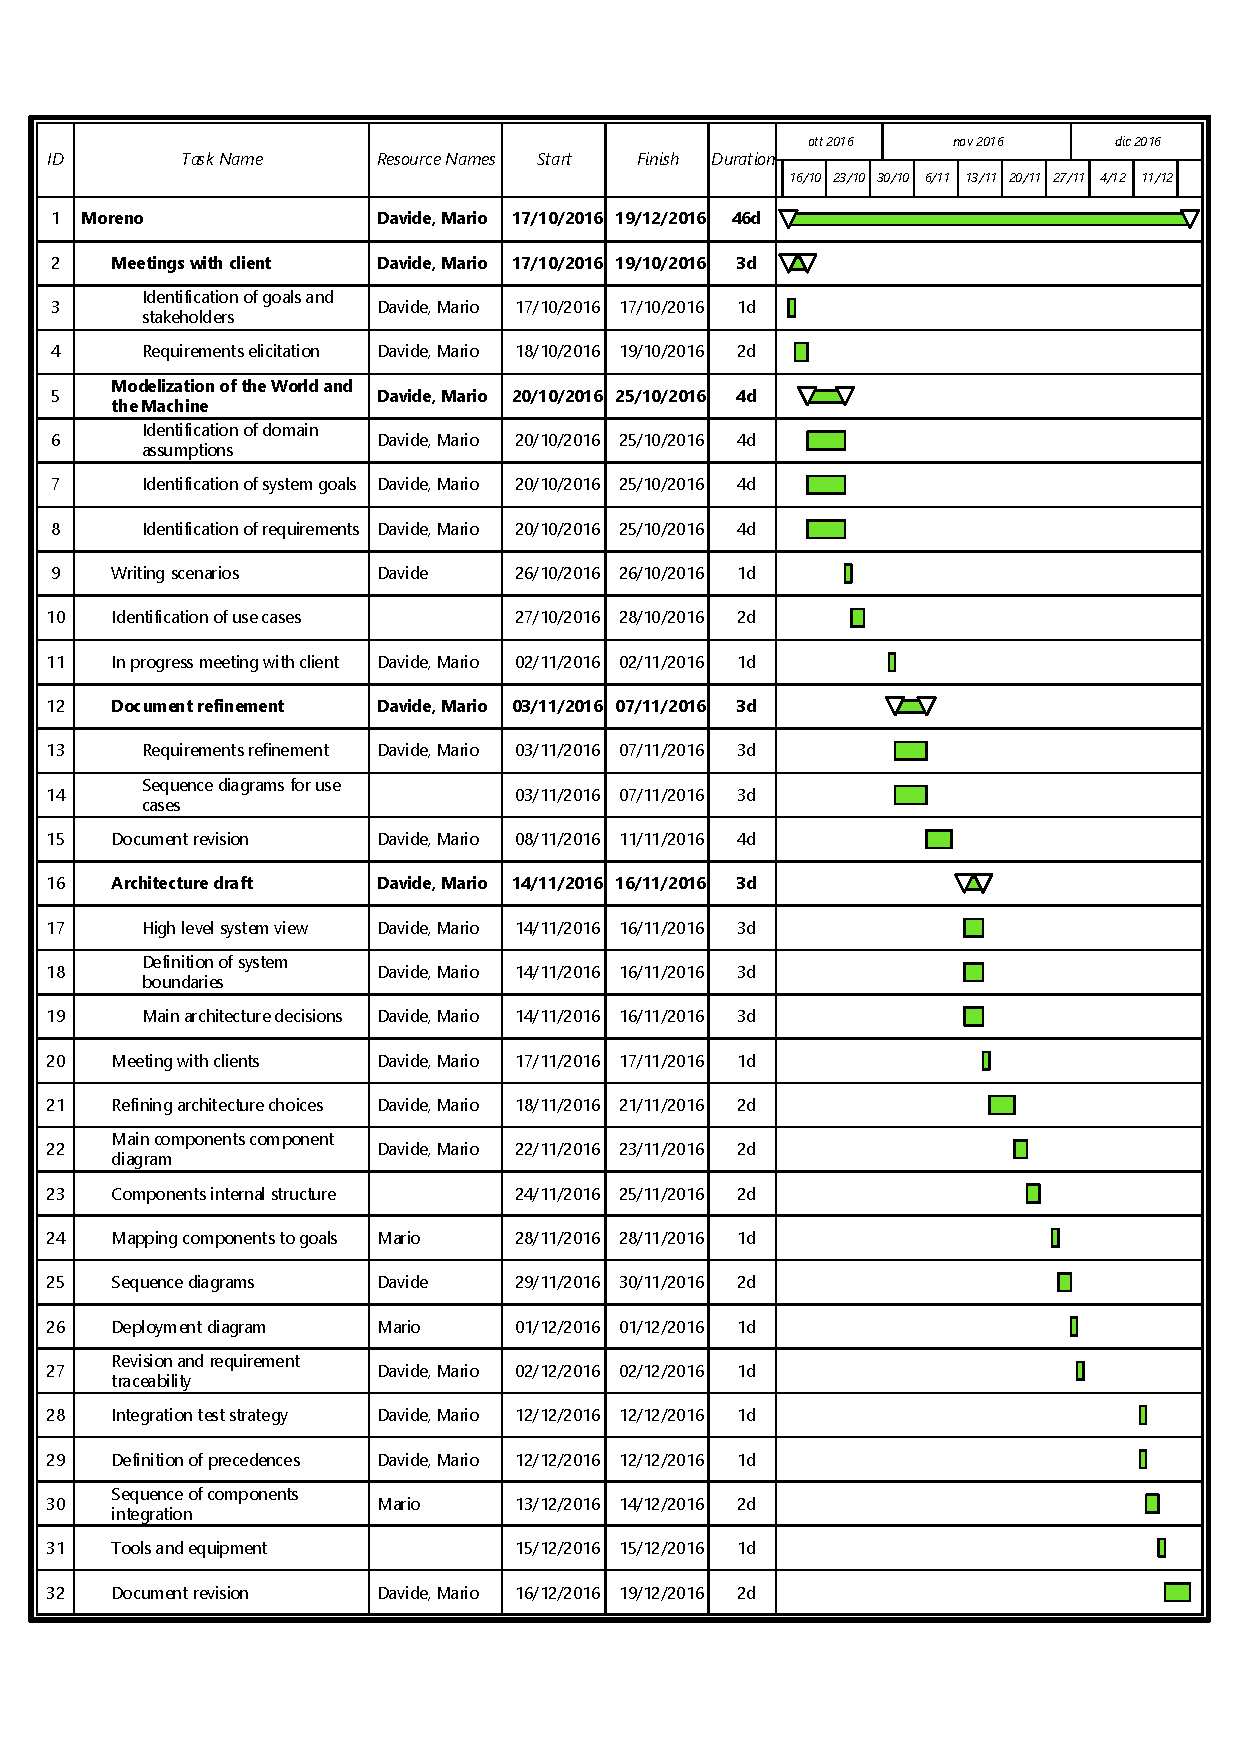
\includegraphics[width=\linewidth]{MorenoGantt}	\caption{
		\label{fig:morenoGantt} 
		Moreno Raimondo Vendra tasks Gantt chart
	}
\end{figure}

\section{Risk management}\label{sec:riskManagement}
This section describe possible risks for the \emph{PowerEnJoy system} and some possible reactive and proactive strategies to mitigate them.
\paragraph{Note} Probability level in ascending order is: 
\begin{enumerate}
\item \emph{Low}
\item \emph{Moderate}
\item \emph{High}
\end{enumerate}
Dangerousness level of effects in ascending order is: \begin{enumerate}
\item \emph{Trivial}
\item \emph{Moderate}
\item \emph{Serious}
\item \emph{Catastrophic}
\end{enumerate}

\subsection{Project risks}
\begin{longtable}{lp{0.8\linewidth}}
\multicolumn{2}{c}{\textbf{Failure to achieve a deadline}}\\
\toprule
\textbf{Description}& Various contingencies could bring to fail to achieve deadlines. \\
\midrule
\textbf{Probability}&Moderate\\
\midrule
\textbf{Effects}&Moderate\\
\midrule
\textbf{Actions}& Considering in the project schedule all the issues that may arise during the project development is definitely a difficult challenge; allocating some extra time after each major phase of the project would help to avoid the shift of some tasks on the schedule because of a missed deadline.\\
\bottomrule
\end{longtable}

\begin{longtable}{lp{0.8\linewidth}}
\multicolumn{2}{c}{\textbf{Change of requirements}}\\
\toprule
\textbf{Description}& Requirements may need some changes for different reasons: not exhaustive requirements, misunderstood requirements or missing requirements. \\
\midrule
\textbf{Probability}&Moderate\\
\midrule
\textbf{Effects}&Moderate/Serious\\
\midrule
\textbf{Actions}& To avoid the need to change requirements it would be really useful to start interacting with all the project stakeholders since the beginning of the project development (for example also allowing some users to interact with mockups of the application during the requirements design phase). 

The change of requirements during the development phase could bring to the need to change already implemented software and/or software design. The relevance on the project of that change must be evaluated. If the issue is serious and is customer fault it could be necessary to re-discuss project contract, schedule and estimated budget. 

Anyway a modular and reusable thinking of the software architecture could help to be more reactive to the need of change some requirements.\\
\bottomrule
\end{longtable}

\begin{longtable}{lp{0.8\linewidth}}
\multicolumn{2}{c}{\textbf{Personnel shortfall}}\\
\toprule
\textbf{Description}& Some member of the development team may leave the project; since the size of the team is quite small it may cause serious effects. \\
\midrule
\textbf{Probability}&Low\\
\midrule
\textbf{Effects}&Serious\\
\midrule
\textbf{Actions}& In order to prevent serious effect multiple the project must be well documented in each phase, meetings must be organized to allow each member of the group to have a general knowledge of each part of the project and critic tasks must not be assigned to a single team member.\\
\bottomrule
\end{longtable}


\subsection{Technical risks}
\begin{longtable}{lp{0.8\linewidth}}
\multicolumn{2}{c}{\textbf{Underestimation of requests' load}}\\
\toprule
\textbf{Description}&Traffic and requests are much more than what has been estimated, resulting in high latency and possibly in service unavailability\\
\midrule
\textbf{Probability}&Low\\
\midrule
\textbf{Effects}&Serious\\
\midrule
\textbf{Actions}&Analyze the traffic through all component, consider an upgrade of hardware components, external API contracts and traffic plans. During the development use a modular software design to manage multiple requests in parallel and to improve scalability.\\
\bottomrule
\end{longtable}

\begin{longtable}{lp{0.8\linewidth}}
\multicolumn{2}{c}{\textbf{Data Loss}}\\
\toprule
\textbf{Description}&Data of the system may be compromised due to an hardware fault or to wrong writing operations.\\
\midrule
\textbf{Probability}&Low\\
\midrule
\textbf{Effects}&Catastrophic\\
\midrule
\textbf{Actions}&It is convenient to store an updated backup copy of data possibly on a different location from the system database one.\\
\bottomrule
\end{longtable}

\begin{longtable}{lp{0.8\linewidth}}
\multicolumn{2}{c}{\textbf{Wrong external component specification}}\\
\toprule
\textbf{Description}&An external component is not compliant to its specification\\
\midrule
\textbf{Probability}&Low\\
\midrule
\textbf{Effects}&Serious\\
\midrule
\textbf{Actions}&Try to find a solution with the component's owner, if impossible find a different compatible component and consider to take legal proceedings.\\
\bottomrule
\end{longtable}

\begin{longtable}{lp{0.8\linewidth}}
\multicolumn{2}{c}{\textbf{Difficulties during development phase}}\\
\toprule
\textbf{Description}& It could happen developers experience difficulties in the development of some specific features of the system due to the lack of experience. \\
\midrule
\textbf{Probability}&Low\\
\midrule
\textbf{Effects}&Moderate\\
\midrule
\textbf{Actions}& It may be required to think about asking consulting to external companies.\\
\bottomrule
\end{longtable}

\begin{longtable}{lp{0.8\linewidth}}
\multicolumn{2}{c}{\textbf{Car supplier changes}}\\
\toprule
\textbf{Description}& It could happen the company for some reason needs to change the car supplier. Since our system relies on the car embedded system provided from our supplier it would be a considerable risk if the system must change the communication protocol used with cars. \\
\midrule
\textbf{Probability}&Low\\
\midrule
\textbf{Effects}&Serious\\
\midrule
\textbf{Actions}& To mitigate the possible effects of this situation the system software must abstract from the type of communication protocol used with cars and interface components must be designed to be as reusable as possible in order to reduce to minimum needed changes.\\
\bottomrule
\end{longtable}

\begin{longtable}{lp{0.8\linewidth}}
\multicolumn{2}{c}{\textbf{External APIs bad behaviour}}\\
\toprule
\textbf{Description}& The system needs to interact with some external APIs that can not behave as expected. \\
\midrule
\textbf{Probability}&Low\\
\midrule
\textbf{Effects}&Moderate\\
\midrule
\textbf{Actions}& External APIs interaction must be deeply tested during the development phase in order to identify possibly unexpected behaviours in this phase: company owner of the API service could be contacted to eventually ask to fix the behaviour or, if it is related to an open source project, a pull request may be proposed to fix the behaviour. \\
\bottomrule
\end{longtable}

\begin{longtable}{lp{0.8\linewidth}}
\multicolumn{2}{c}{\textbf{External APIs downtime}}\\
\toprule
\textbf{Description}& The external APIs the system has to interact with may be unreachable.\\
\midrule
\textbf{Probability}&Low/Moderate\\
\midrule
\textbf{Effects}&Serious\\
\midrule
\textbf{Actions}& Always try to provide as many functionality as possible: if the failure is not in a core functionality, e.g. payments API fails, it would be useful to develop the system such that it is possible to keep the whole system online and operative and at the same time store the unprocessed payments for future proceeding.

When it is possible take into account the usage of redundant APIs according to failure recovery paradigms. \\
\bottomrule
\end{longtable}

\subsection{Business risks}
\begin{longtable}{lp{0.8\linewidth}}
\multicolumn{2}{c}{\textbf{Competitors}}\\
\toprule
\textbf{Description}&Competitors saturate the market with their car sharing services\\
\midrule
\textbf{Probability}&High\\
\midrule
\textbf{Effects}&Serious\\
\midrule
\textbf{Actions}&Make some market surveys in order to determine and implement some \emph{killer features} to persuade users to use the \emph{PowerEnJoy} service.\\
\bottomrule
\end{longtable}

\begin{longtable}{lp{0.8\linewidth}}
\multicolumn{2}{c}{\textbf{Financial crisis}}\\
\toprule
\textbf{Description}&Customer may have financial troubles during the development of the system causing a reduction of the budget.\\
\midrule
\textbf{Probability}&Low\\
\midrule
\textbf{Effects}&Catastrophic\\
\midrule
\textbf{Actions}& A good study of feasibility would detect this risk.  This situation could be mitigate meeting the customer and re-discussing features and agreed requirements but could also bring to the end of the project development. \\
\bottomrule
\end{longtable}



\begin{appendices}

	\section{Software and tools used}
	For the development of this document we used
	\begin{itemize}
		\item \LaTeX{} as document preparation system
		\item Git \& \href{http://github.com}{GitHub} as version control system
		\item Microsoft Visio and Excel as Gantt diagrams generators
	\end{itemize}
	
	\section{Hours of work}
	This is the amount of time spent to redact this document:
	\begin{itemize}
		\item Davide Piantella: $\sim$ 18 hours
		\item Mario Scrocca: $\sim$ 16 hours
		\item Moreno R. Vendra: $\sim$ 14 hours
	\end{itemize}
	
\end{appendices}


\begin{thebibliography}{9}

\bibitem{RASD}D. Piantella, M. Scrocca, M.R. Vendra, \emph{PowerEnJoy: Requirements Analysis and Specification Document}, Politecnico di Milano - Software Engineering II Project, 2016

\bibitem{DD}D. Piantella, M. Scrocca, M.R. Vendra, \emph{PowerEnJoy: Design Document}, Politecnico di Milano - Software Engineering II Project, 2016

\bibitem{ITPD}D. Piantella, M. Scrocca, M.R. Vendra, \emph{PowerEnJoy: Integration Test Plan Document}, Politecnico di Milano - Software Engineering II Project, 2017

\bibitem{QSM}Quantitative Software Management, Function Point Languages Table version 5.0, QSM SLOC/FP Data, \url{http://www.qsm.com/resources/function-point-languages-table}

\bibitem{FP}International Function Point Users Group (IFPUG),
\\\emph{Function Point Counting Practices Manual}, Release 4.2 

\bibitem{COCOMO}University of Southern California, Center for Systems and Software Engineering, \emph{COCOMO II}, \url{http://csse.usc.edu/csse/research/COCOMOII/cocomo_main.html}

\bibitem{COCOMOManual}University of Southern California, Center for Systems and Software Engineering, \emph{COCOMO II.2000 Model Definition Manual}, \url{http://csse.usc.edu/csse/research/COCOMOII/cocomo2000.0/CII_modelman2000.0.pdf}

\end{thebibliography}

\end{document}